% =============================================================================
% The CGAL User Manual
% Chapter: Geometric Optimisation
% Section: QP solver
% =============================================================================
\newcommand{\qprel}{\ccTexHtml{\gtreqless}{&nbsp;~&nbsp;}}

\ccUserChapter{QP\_solver}\label{QP_solver}
\ccChapterRelease{Release: WIP (\today)}
\ccChapterAuthor{Kaspar Fischer \and Bernd G{\"a}rtner 
\and Sven Sch{\"o}nherr \and Frans Wessendorp}

\section{A first quadratic program}
This section explains what linear and quadratic programs are, gives a
simple example of a quadratic program, and shows how CGAL can be used
to solve it.

\subsection{Quadratic programs}
This package lets you solve \emph{convex quadratic programs} of the 
general form
\begin{eqnarray*}
\mbox{(QP)}&\mbox{minimize} & x^{T}Dx + c^{T}x + c_0 \\
&\mbox{subject to}   & Ax\qprel b, \\
&& l \leq x \leq u
\end{eqnarray*}
over $n$ variables $x=(x_0,\ldots,x_{n-1})$.

Here, $A \in \R^{m \times n}$ is the \emph{constraint matrix} and $b
\in \R^{m}$ the \emph{right-hand} side. The symbol ``$\qprel$'' in the
program's set $Ax \qprel b$ of $m$ \emph{constraints} indicates that for
$i=1,\ldots,m$, the $i$-th constraint may either be an inequality
$(Ax)_i \leq b_i$ or $(Ax)_i \geq b_i$, or an equality $(Ax)_i = b_i$.

Furthermore, $l\in
(\R\cup\{-\infty\})^n$ and $r\in (\R\cup\{\infty\})^n$ are \emph{bounds}
for the variables. Consequently, each
variable $x_j$, $j\in\{0,\ldots,n-1\}$, can be \emph{free} (if
$l_j=-\infty$ and $r_j=\infty$), \emph{upper-bounded} (if
$u_j\neq\infty$) and/or \emph{lower-bounded} (if
$l_j\neq-\infty)$.  

$D \in \R^{n \times n}$ is the \emph{quadratic
objective function matrix}. $D$ must be symmetric and 
positive-semidefinite in order for the \emph{quadratic objective function}
$x^{T}Dx$ to be convex. $c \in \R^{n}$ is the \emph{linear
objective function}, and $c_0$ is the \emph{constant term}. The full
\emph{objective function} is the sum of the quadratic, the linear, and
the constant term.

\emph{Solving} the quadratic program means to find a vector $x^*$ such
that $Ax^*\qprel b, l\leq x^*\leq u$ (a \emph{feasible solution}) with
the smallest objective function value among all feasible solutions.
Such a solution may not exist, see Sections
\ref{sec:QP-infeasible} and \ref{sec:QP-unbounded} below.

\subsection{Linear and nonnegative programs.}
If $D=0$, the quadratic program is in fact a \emph{linear program},
and in the case that $l$ is the zero vector and all entries of
$u$ are $\infty$, the program is said to be \emph{nonnegative}. The 
package offers dedicated solution methods for these special cases,
see Sections \ref{sec:QP-lp} and \ref{sec:QP-nonnegative} below.

\subsection{A first example}
Let's consider the following quadratic program in two variables:
\[
\begin{array}{lrcl}
\mbox{minimize}       & x^2 + 4(y-4)^2 &(=& x^2 + 4y^2 - 32y + 64) \\
\mbox{subject to}     & x + y &\leq& 7 \\
                      & -x + 2y &\leq& 4 \\
                      & x &\geq& 0 \\
                      & y &\geq& 0 \\
                      & y &\leq& 4
\end{array}
\]

Figure \ref{fig:QP-first_qp} shows a planar drawing of this. The figure
depicts the five inequalities of the program, along with the
\emph{feasible region} (green), the set of points that satisfy all the
five constraints. The dashed elliptic curves represent \emph{contour lines} 
of the objective function, i.e. along each dashed curve, the objective
function value is constant. 

The global minimum of the objective function is attained at 
the point $(0,4)$, and the minimum within the feasible region appears
at the point $(2,3)$ marked with a black dot. The value of the objective
function at this optimal solution is $2^2 + 4(3-4)^2 = 8$.

\begin{figure}[htbp]
\begin{ccTexOnly}
\begin{center}
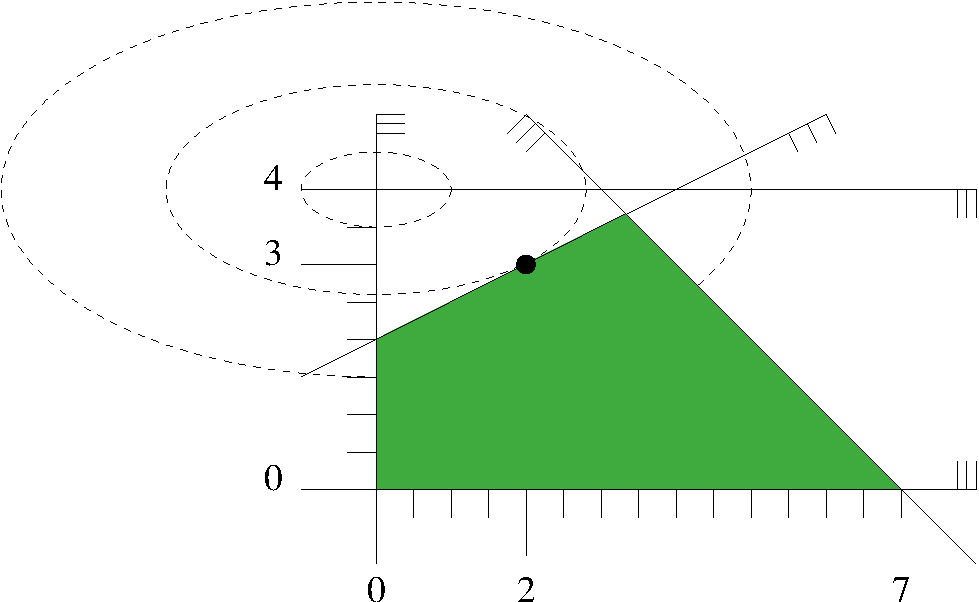
\includegraphics{QP_solver/first_qp} % omit suffix .eps to supprt PS and PDF
\end{center}
\end{ccTexOnly}
\caption{A quadratic program in two variables
\label{fig:QP-first_qp}}

\begin{ccHtmlOnly}
<CENTER>
<IMG BORDER=0 SRC="./first_qp.gif" ALIGN=center ALT="A quadratic program in two variables">
</CENTER>
\end{ccHtmlOnly}
\end{figure}

Here is how this quadratic program can be solved in CGAL (for an example
how to work with \ccc{double} as input type see \ldots)
The output will be:
\begin{verbatim}
Optimal feasible solution: 2/1  3/1
Optimal objective function value: 8/1
\end{verbatim}

\ccIncludeExampleCode{QP_solver/first_qp.cpp}


\section{Which programs can efficiently be solved?}
\label{sec:QP-efficiency}
This can quite precisely be answered in terms of the following
parameters.
\begin{tabular}{lcl}
$n$ &: & the number of variables (or columns of $A$),\\
$m$ &: &the number of constraints (or rows of $A$),\\
$e$ &: &the number of equality constraints,\\
$r$ &: &the rank of the quadratic objective function matrix $D$.
\end{tabular}
The runtime is approximately linear in $\max(n,m)$, 
but with a factor heavily depending on $\min(n,e)+r$.
Therefore, the solver will be efficient only if $\min(n,e)+r$ is small.

Here are the scenarios in which this applies:
\begin{itemize}
\item Quadratic programs with a small number of variables, but
  possibly a large number of inequality constraints
\item Linear programs with a small number of equality constraints but
  possibly a large number of variables
\item Quadratic programs with a small number of equality constraints and
  $D$ of small rank, but possibly with a large number of variables
\end{itemize} 

How small is small? If $\min(n,e)+r$ is up to $10$, the solver will
probably be very fast, even if $\max(n,m)$ goes into the millions. 
If $\min(n,m)+r$ is up to a few hundreds, you may still get a solution 
within reasonable time, depending on the problem characteristics.

If you have a problem where both $n$ and $e$ are above
$1,000$, say, then chances are high that CGAL cannot solve it.
This even holds if the problem is \emph{sparse}, i.e. has a small
number of nonzero elements in $A$ and $D$. CGAL's quadratic programming
solver is tailored to \emph{dense} problems and therefore does not 
profit from sparse input.

\section{How robust is the solver?}
Given that you use an \emph{exact number type} for the 
calculations (as in the example program above), the solver
will give you \emph{exact rational output}, for \emph{every}
convex quadratic program. This means, there are no robustness
issues with the solver. Not taking bugs into account, the solver 
may fail to compute a solution only if
\begin{itemize}
\item the quadratic program is too large (see previous Section 
\ref{sec:QP-efficiency}), 
\item the quadratic objective function matrix $D$ is not 
positive-semidefinite, or
\item the solver internally cycles. This may happen in very rare
cases (so rare actually that it does not pay off to take
precautions against internal cycling by default). However, if
you have a hunch that the solver cycles on your problem,
there are means to switch to a slower variant that is guaranteed
not to cycle, see\ldots 
\end{itemize}

\section{Linear programs}\label{sec:QP-lp}
You can solve a linear program by solving a quadratic program with
quadratic objective function matrix $D=0$. But there is a more efficient
dedicated function for solving a linear program that also saves you
from providing $D$ in the first place. 

Let's go back to our first quadratic program from above and change it 
into a linear program by simply removing the quadratic part of the
objective function:

\[
\begin{array}{lrcl}
\mbox{minimize}       & - 32y + 64 \\
\mbox{subject to}     & x + y &\leq& 7 \\
                      & -x + 2y &\leq& 4 \\
                      & x &\geq& 0 \\
                      & y &\geq& 0 \\
                      & y &\leq& 4
\end{array}
\] 

Figure \ref{fig:QP-first_lp} shows how this looks like. We will not
visualize a linear objective function with contour lines but with
arrows instead. The arrow represents the (direction) of the vector $-c$,
and we are looking for a feasible solution that is ``extreme'' in the direction
of the arrow. In our small example, this is the unique point ``on'' the
two constraints $x_1+x_2\leq 7$ and $-x_1+x_2\leq 4$, the point
$(10/3,11/3)$ marked with a black dot. The optimal objective function
value is $-32(11/3)+64=-160/3$.

\begin{figure}[htbp]
\begin{ccTexOnly}
\begin{center}
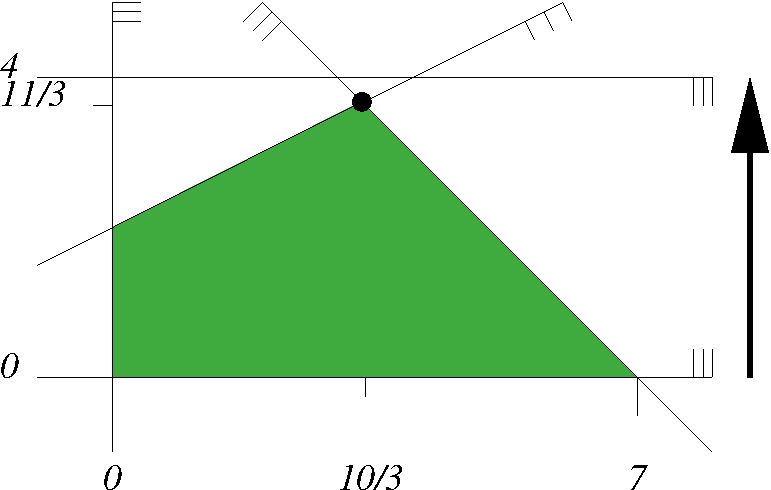
\includegraphics{QP_solver/first_lp} % omit suffix .eps to supprt PS and PDF
\end{center}
\end{ccTexOnly}
\caption{A linear program in two variables
\label{fig:QP-first_lp}}

\begin{ccHtmlOnly}
<CENTER>
<IMG BORDER=0 SRC="./first_lp.gif" ALIGN=center ALT="A linear program in two variables">
</CENTER>
\end{ccHtmlOnly}
\end{figure}

Here is a CGAL code for solving it. Its output is
\begin{verbatim}
Optimal feasible solution: 10/3  11/3
Optimal objective function value: -160/3
\end{verbatim}

\ccIncludeExampleCode{QP_solver/first_lp.cpp}

\section{Nonnegative programs}\label{sec:QP-nonnegative}

Often, the bounds in a quadratic or linear program are of the special
type $x\geq 0$. Programs of this type are called nonnegative and
can be solved by dedicated CGAL functions. This is more efficient than
calling the general functions, and it saves you from providing any bound
information at all. If we go back to our first quadratic program and
remove the constraint $y\leq 4$, we arrive at a nonnegative quadratic
program: 

\[
\begin{array}{lrcl}
\mbox{minimize}       & x^2 + 4(y-4)^2 &(=& x^2 + 4y^2 - 32y + 64) \\
\mbox{subject to}     & x + y &\leq& 7 \\
                      & -x + 2y &\leq& 4 \\
                      & x,y &\geq& 0
\end{array}
\]

Figure \ref{fig:QP-first_nonnegative_qp} contains 
the planar illustration; since the constraint $y\leq 4$ was 
redundant, the feasible region and the optimal solution do 
not change. 

\begin{figure}[htbp]
\begin{ccTexOnly}
\begin{center}
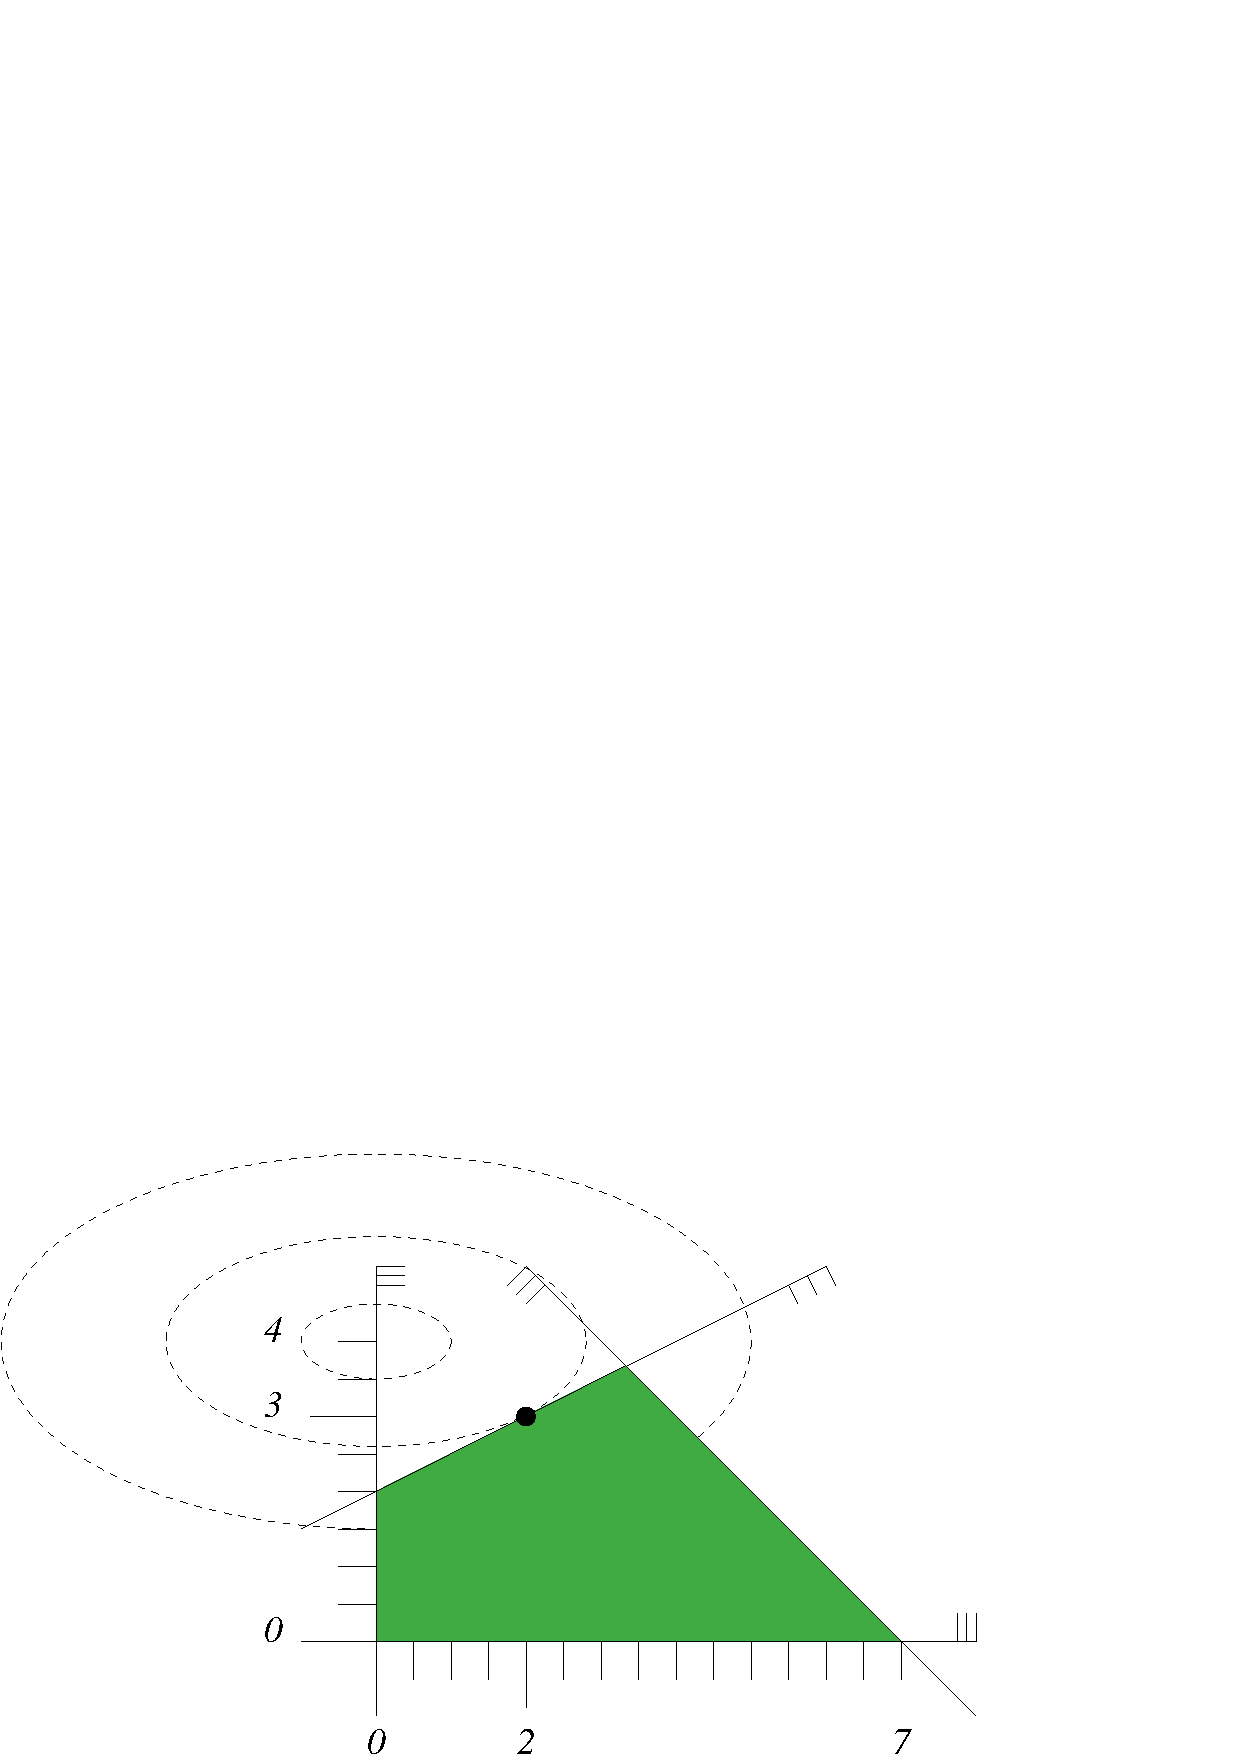
\includegraphics{QP_solver/first_nonnegative_qp} 
\end{center}
\end{ccTexOnly}
\caption{A nonnegative quadratic program in two variables
\label{fig:QP-first_nonnegative_qp}}

\begin{ccHtmlOnly}
<CENTER>
<IMG BORDER=0 SRC="./first_nonnegative_qp.gif" ALIGN=center ALT="A linear program in two variables">
</CENTER>
\end{ccHtmlOnly}
\end{figure}

The following program will therefore again output
\begin{verbatim}
Optimal feasible solution: 2/1  3/1
Optimal objective function value: 8/1
\end{verbatim}

\ccIncludeExampleCode{QP_solver/first_nonnegative_qp.cpp}

Finally, a dedicated function is available for nonnnegative linear
programs as well. Let's take our linear program from above and remove
the constraint $y\leq 4$ to obtain a nonnegative linear program. At
the same time we remove the constant objective function term to get
a ``minimal'' input and a ``shortest'' program; the optimal value is
$-32(11/3)=-352/3$.

\[
\begin{array}{lrcl}
\mbox{minimize}       & - 32y \\
\mbox{subject to}     & x + y &\leq& 7 \\
                      & -x + 2y &\leq& 4 \\
                      & x,y &\geq& 0 \\
\end{array}
\] 

This can be solved as follows; the output is
\begin{verbatim}
Optimal feasible solution: 10/3  11/3
Optimal objective function value: -352/3
\end{verbatim}

\ccIncludeExampleCode{QP_solver/first_nonnegative_lp.cpp}

\section{The solution}

\section{Infeasibility}\label{sec:QP-infeasible}

\section{Unboundedness}\label{sec:QP-unbounded}

\section{The important variables}

\section{The important constraints}

\section{Certificates for the solution}

\section{Solving linear and quadratic programs from MPS files}



